\chapter{Theory}\label{chap:cms}



\section{The Standard Model}

The Standard Model (SM) describes the fundamental particles and forces (excluding gravity) using Quantum Field Theory (QFT).


\subsection{Fundamental Particles}

The fundamental particles in the standard model are shown in Figure~\ref{fig:sm}.

\begin{figure}[h]
	\centering
	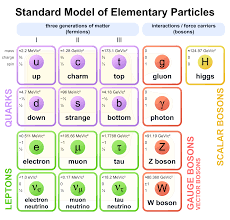
\includegraphics[width=0.7\textwidth]{figures/sm_blocks.png}
	\caption{The fundamental particles in the standard model of particle physics~\cite{StandardModel}.}
	\label{fig:sm}
\end{figure}



Fundamental particles are particles with no substructure. They are point particles with properties such as mass and spin. In the standard model, there are 17 fundamental particles. Of these, 12 are fermions - spin-1/2 particles - and 5 are bosons - integer-spin particles. 

The fermions are further classified into "quarks" and "leptons". Quarks have electromagnetic charge and color charge. Leptons have electroweak charge only. The properties of the leptons are described in Table~\ref{tab:leptons}, and the properties of the quarks are described in Table~\ref{tab:quarks}. 





Particles interact by exchanging force particles, all of which are spin-1 bosons in the Standard Model~\cite{martin}.


\begin{table}
\begin{center}
\begin{tabular}{||c c r c||} 
 \hline
 Particle & Mass [MeV] & Charge & Lifetime \\ [0.5ex] 
 \hline\hline
 $e^{-}$ & $0.511$ & $-1$ & Stable \\ 
 \hline
 $\nu_e$ & $<2$ & $0$ & Stable \\
 \hline
 $\mu^{-}$ & $105.7$ & $-1$ & $2.197 \times 10^{-6}$ \\
 \hline
 $\nu_\mu$ & $<0.19$ & $0$ & Stable \\
 \hline
 $\tau^{-}$ & $1777$ & $-1$ & $2.906 \times 10^{-13}$  \\
 \hline
 $\nu_\tau$ & $<18.2$ & $0$ & Stable \\ [1ex] 
 \hline
\end{tabular}
\end{center}
\caption{Mass, charge and lifetime of the leptons and lepton neutrinos~\cite{martin}.}
\label{tab:leptons}
\end{table}

\begin{table}
\begin{center}
\begin{tabular}{||c c r c||} 
 \hline
 Particle & Mass [GeV] & Charge & Lifetime \\ [0.5ex] 
 \hline\hline
 $u$ & $0.3$ & $2/3$ & Stable \\ 
 \hline
 $d$ & $0.3$ & $-1/3$ & Stable \\
 \hline
 $c$ & $1.5$ & $2/3$ & $10^{-12}$ \\
 \hline
 $s$ & $0.5$ & $-1/3$ & $10^{-8}$ \\
 \hline
 $t$ & $173$ & $2/3$ & $10^{-25}$  \\
 \hline
 $b$ & $4.5$ & $-1/3$ & $10^{-12}$ \\ [1ex] 
 \hline
\end{tabular}
\end{center}
\caption{Mass, charge and lifetime of the quarks~\cite{martin}.}
\label{tab:quarks}
\end{table}


The fermions are categorized into three generations; the first generation is represented by the first column in Figure~\ref{fig:sm}, the second generation is represented by the second row, and the third generation is represented by the third row. The generations are ordered by the masses of the quarks and leptons, and so the heavier generations can decay to the lighter generations, for example a muon can decay to an electron:

\begin{equation}
	\mu^{-} \rightarrow e^{-} + \bar{\nu}_e + \nu_\mu
\end{equation}

 The first generation particles do not have any known decays.


\subsection{Standard Model Forces}

The fermions interact with one another by exchanging spin-1 gauge bosons - the force carrying particles. The strong force is mediated by the gluon, the electromagnetic force is mediated by the photon, and the weak force is mediated by the $Z^0$ and $W^{\pm}$ bosons. 

\subsection*{Strong Force}

The strong force is described by Quantum Chromodynamics (QCD). QCD is a form of QFT with symmetry group SU(3). The force carriers, the gluons, are neutral particles that carry the color charge. There are three possible color charges: red, green, and blue. QCD obeys "color confinement", in which only color-neutral particles can exist. Color neutrality can be achieved by combing a red, green, and blue quark, or by combining a quark and anti quark of the same color (e.g. red and anti-red).

The particles in QCD also obey "asymptotic freedom", the property in which the strength of the strong force increases as distance increases. As the distance between the quarks in a $q\bar{q}$ increases, instead of the particles becoming isolated, a new $q\bar{q}$ pair is produced.

A QCD scattering interaction is shown in Figure~\ref{fig:feynman_qq}.

\begin{figure}[h!]
	\centering
	\feynmandiagram [vertical=a to b] {
	  i1 [particle=\(\color{red}{u}\)] -- [fermion] a -- [fermion] i2 [particle=\(\color{blue}{u}\)],
	  a -- [gluon, edge label'=\(g\)] b,
 	 f1 [particle=\(\color{red}{s}\)] -- [anti fermion] b -- [anti fermion] f2 [particle=\(\color{blue}{s}\)],
	};
	\caption{$qq$ scattering with an up quark with red color charge and a strange quark with blue color charge.}
	\label{fig:feynman_qq}
\end{figure} 



\subsection*{Electromagnetic Force}

The electromagnetic force is mediated by the photon, which carries the electric charge ($\pm 1$) and only acts on charged particles. The electromagnetic force is described by Quantum Electrodynamics (QED), which has a coupling strength $\alpha \approx 1/137$. In QED, particles obey the "Pauli Exclusion Principle": no two fermions can inhabit the same quantum state. An electromagnetic scattering interaction is shown in Figure~\ref{fig:feynman_ee}.

\begin{figure}[h]
	\centering
	\feynmandiagram [vertical=a to b] {
	  i1 [particle=\(e^{-}\)] -- [fermion] a -- [fermion] i2 [particle=\(e^{-}\)],
	  a -- [photon, edge label'=\(\gamma\)] b,
 	 f1 [particle=\(\mu^{-}\)] -- [anti fermion] b -- [anti fermion] f2 [particle=\(\mu^{-}\)],
	};
	\caption{An electron muon scattering interaction with scattering amplitude $e^2/q^2$ for a 1 photon exchange interaction.}
	\label{fig:feynman_ee}
\end{figure}



\subsection*{Weak Force}

All fermions can interact through the weak force. The weak force is so named because it is the weakest of the three standard model forces with a coupling strength $a_W \approx 10^{-6}$ (gravity, which is not in the standard model, is weaker than the weak force). Lepton neutrinos interact through the weak force only.




\section{Electroweak Symmetry Breaking}

The electroweak interaction is a unified description of the electromagnetic and weak forces. It is based on the symmetry groups $SU(2)_L \times U(1)_Y$. At high temperatures corresponding to an energy of 246 GeV, the electromagnetic and weak forces can be described by one force. Experiments finding the W and Z bosons confirmed some of the predictions of the theory. The electroweak force has four bosons before symmetry breaking occurs ($W_1$, $W_2$, $W_3$ and $B$). After electroweak symmetry breaking, the $W$ boson is a combination of the first 2 electroweak bosons (Equation~\ref{eq:w}) and the photon and $W$ and $Z$ bosons are a combination of the latter 2 (Equation~\ref{eq:zgamma})

\begin{equation}
	W^{\pm} = \frac{1}{\sqrt{2}}
	\begin{pmatrix}
		W_1 \mp iW_2
	\end{pmatrix}
	\label{eq:w}
\end{equation}


\begin{equation}
	\begin{pmatrix}
		\gamma \\
		Z 
	\end{pmatrix} = \begin{pmatrix}
		\cos{\theta_W} & \sin{\theta_W} \\
		-\sin{\theta_W} & \cos{\theta_W}
	\end{pmatrix}
	\begin{pmatrix}
		B \\
		W_3 
	\end{pmatrix}
	\label{eq:zgamma}
\end{equation}

where $\theta_W$ is the weak mixing angle, or "Weinberg angle", which is the angle relating $g'$ to $g$, the hypercharge and isospin, respectively, of the weak interaction (see Figure~\ref{fig:weinberg}).

\begin{figure}[htbp!]
	\centering
	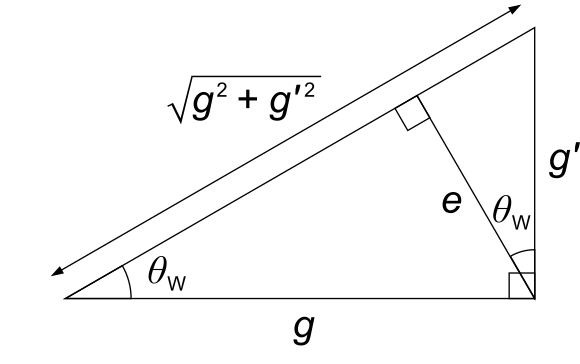
\includegraphics[width=0.4\textwidth]{figures/Weinberg_angle.png}
	\caption{The weak mixing angle $\theta_W$ is the angle relating $g'$ to $g$.}
	\label{fig:weinberg}
\end{figure}


\subsection*{Higgs Mechanism}

The Higgs boson, the spin-0 scalar boson of the standard model, is responsible for electroweak symmetry breaking through the "Higgs Mechanism". The Higgs Mechanism is the term for the $SU(2)_L \times U(1)_Y$ symmetry of the electroweak force breaking into the the $U(1)$ of the electromagnetic force.


The Higgs Mechanism was proposed in 1964~\cite{higgs}. Collider experiments since searched for the Higgs particle, whose mass was not known from theoretical predictions. The Higgs boson was not detected until 2012, when the CMS and ATLAS experiments at the LHC published separate 


\section{Beyond the Standard Model}


The Standard Model is incomplete. It does not contain gravity, which is much weaker than the weak force. The matter described by the standard model makes up only 5\% of the known matter in the universe, the rest is Dark Matter (matter that does not interact with Standard Model particles but does interact gravitationally) and Dark Energy, which is responsible for the acceleration of the expansion of the universe. Theoretical models attempt to solve these problems. 


\subsection*{Extra Dimensions}


\begin{figure}[h!]
	\centering
	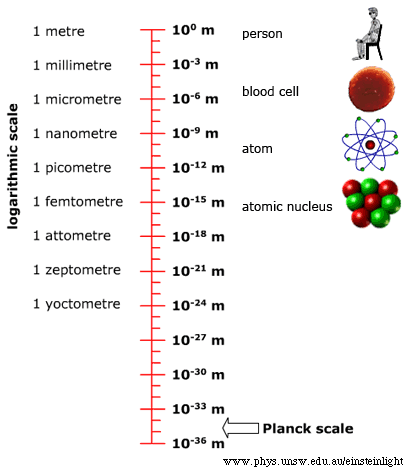
\includegraphics[width=0.5\textwidth]{figures/Planck_scale.png}
	\caption{Logarithmic scale of standard model forces and Planck scale~\cite{Planck_scale}.}
	\label{fig:planck}
\end{figure}


The orders of magnitude difference between the Planck scale and the electroweak scale is called the "Hierarchy Problem". Theoretical predictions suggest that the mass of the Higgs boson should be much larger than its $m_H \approx 125$ GeV. The heaviest fundamental particle is the top quark, at $m_t \approx 173$ GeV, which is on the order of the electroweak scale ($\approx 100$ GeV). A possible answer to this discrepancy is to search for new, heavier particles at the highest energy scales possible at the LHC that decay to $t\bar{t}$ pairs. 

The Randall Sundrum (RS1) model is a theoretical framework with a fourth spatial dimension, with a 3 dimensional brane on the electroweak scale and a 1 dimensional brane on the Planck scale~\cite{rs1}. Figure~\ref{fig:rsbrane} shows a diagram of this RS1 model, where the scale of gravity decreases when moving from the UV brane to the IR brane. The model proposes a graviton that is on the TeV scale, and decays to $t\bar{t}$. A second Randall-Sundrum model (RS2) proposes a fourth spatial dimension but only one TeV-scale brane~\cite{rs2}.

\begin{figure}[h]
	\centering
	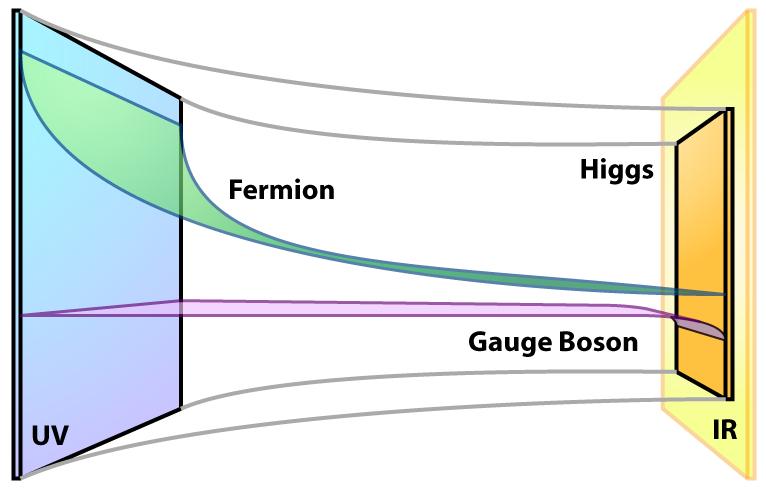
\includegraphics[width=0.75\textwidth]{figures/RSBrane.png}
	\caption{The extra spatial dimensions proposed in the Randall-Sundrum model~\cite{RSBrane}.}
	\label{fig:rsbrane}
\end{figure}



%
%\subsection*{Dark Matter}
%
%
%Simplified Dark Matter models propose a $Z'$ boson that decays to $t\bar{t}$~\cite{simplified_dm}.
%
%
%
\subsection*{$Z'$ Models}

Some models predict exotic $Z'$ bosons that can decay to SM $t\bar{t}$ if the couplings to leptons are suppressed, and $m_{Z'} > 2m_{t}$~\cite{leptophobicZprime}. The leptophobic $Z'$ still decays to exotic leptons $\approx 50$\% of the time.

Simplified Dark Matter (DM) models predict DM particles interacting with SM particles through a $Z'$ mediator boson~\cite{wasmer_dark_matter}.

\section{Monte Carlo Simulation}

\begin{figure}[h]
	\centering
	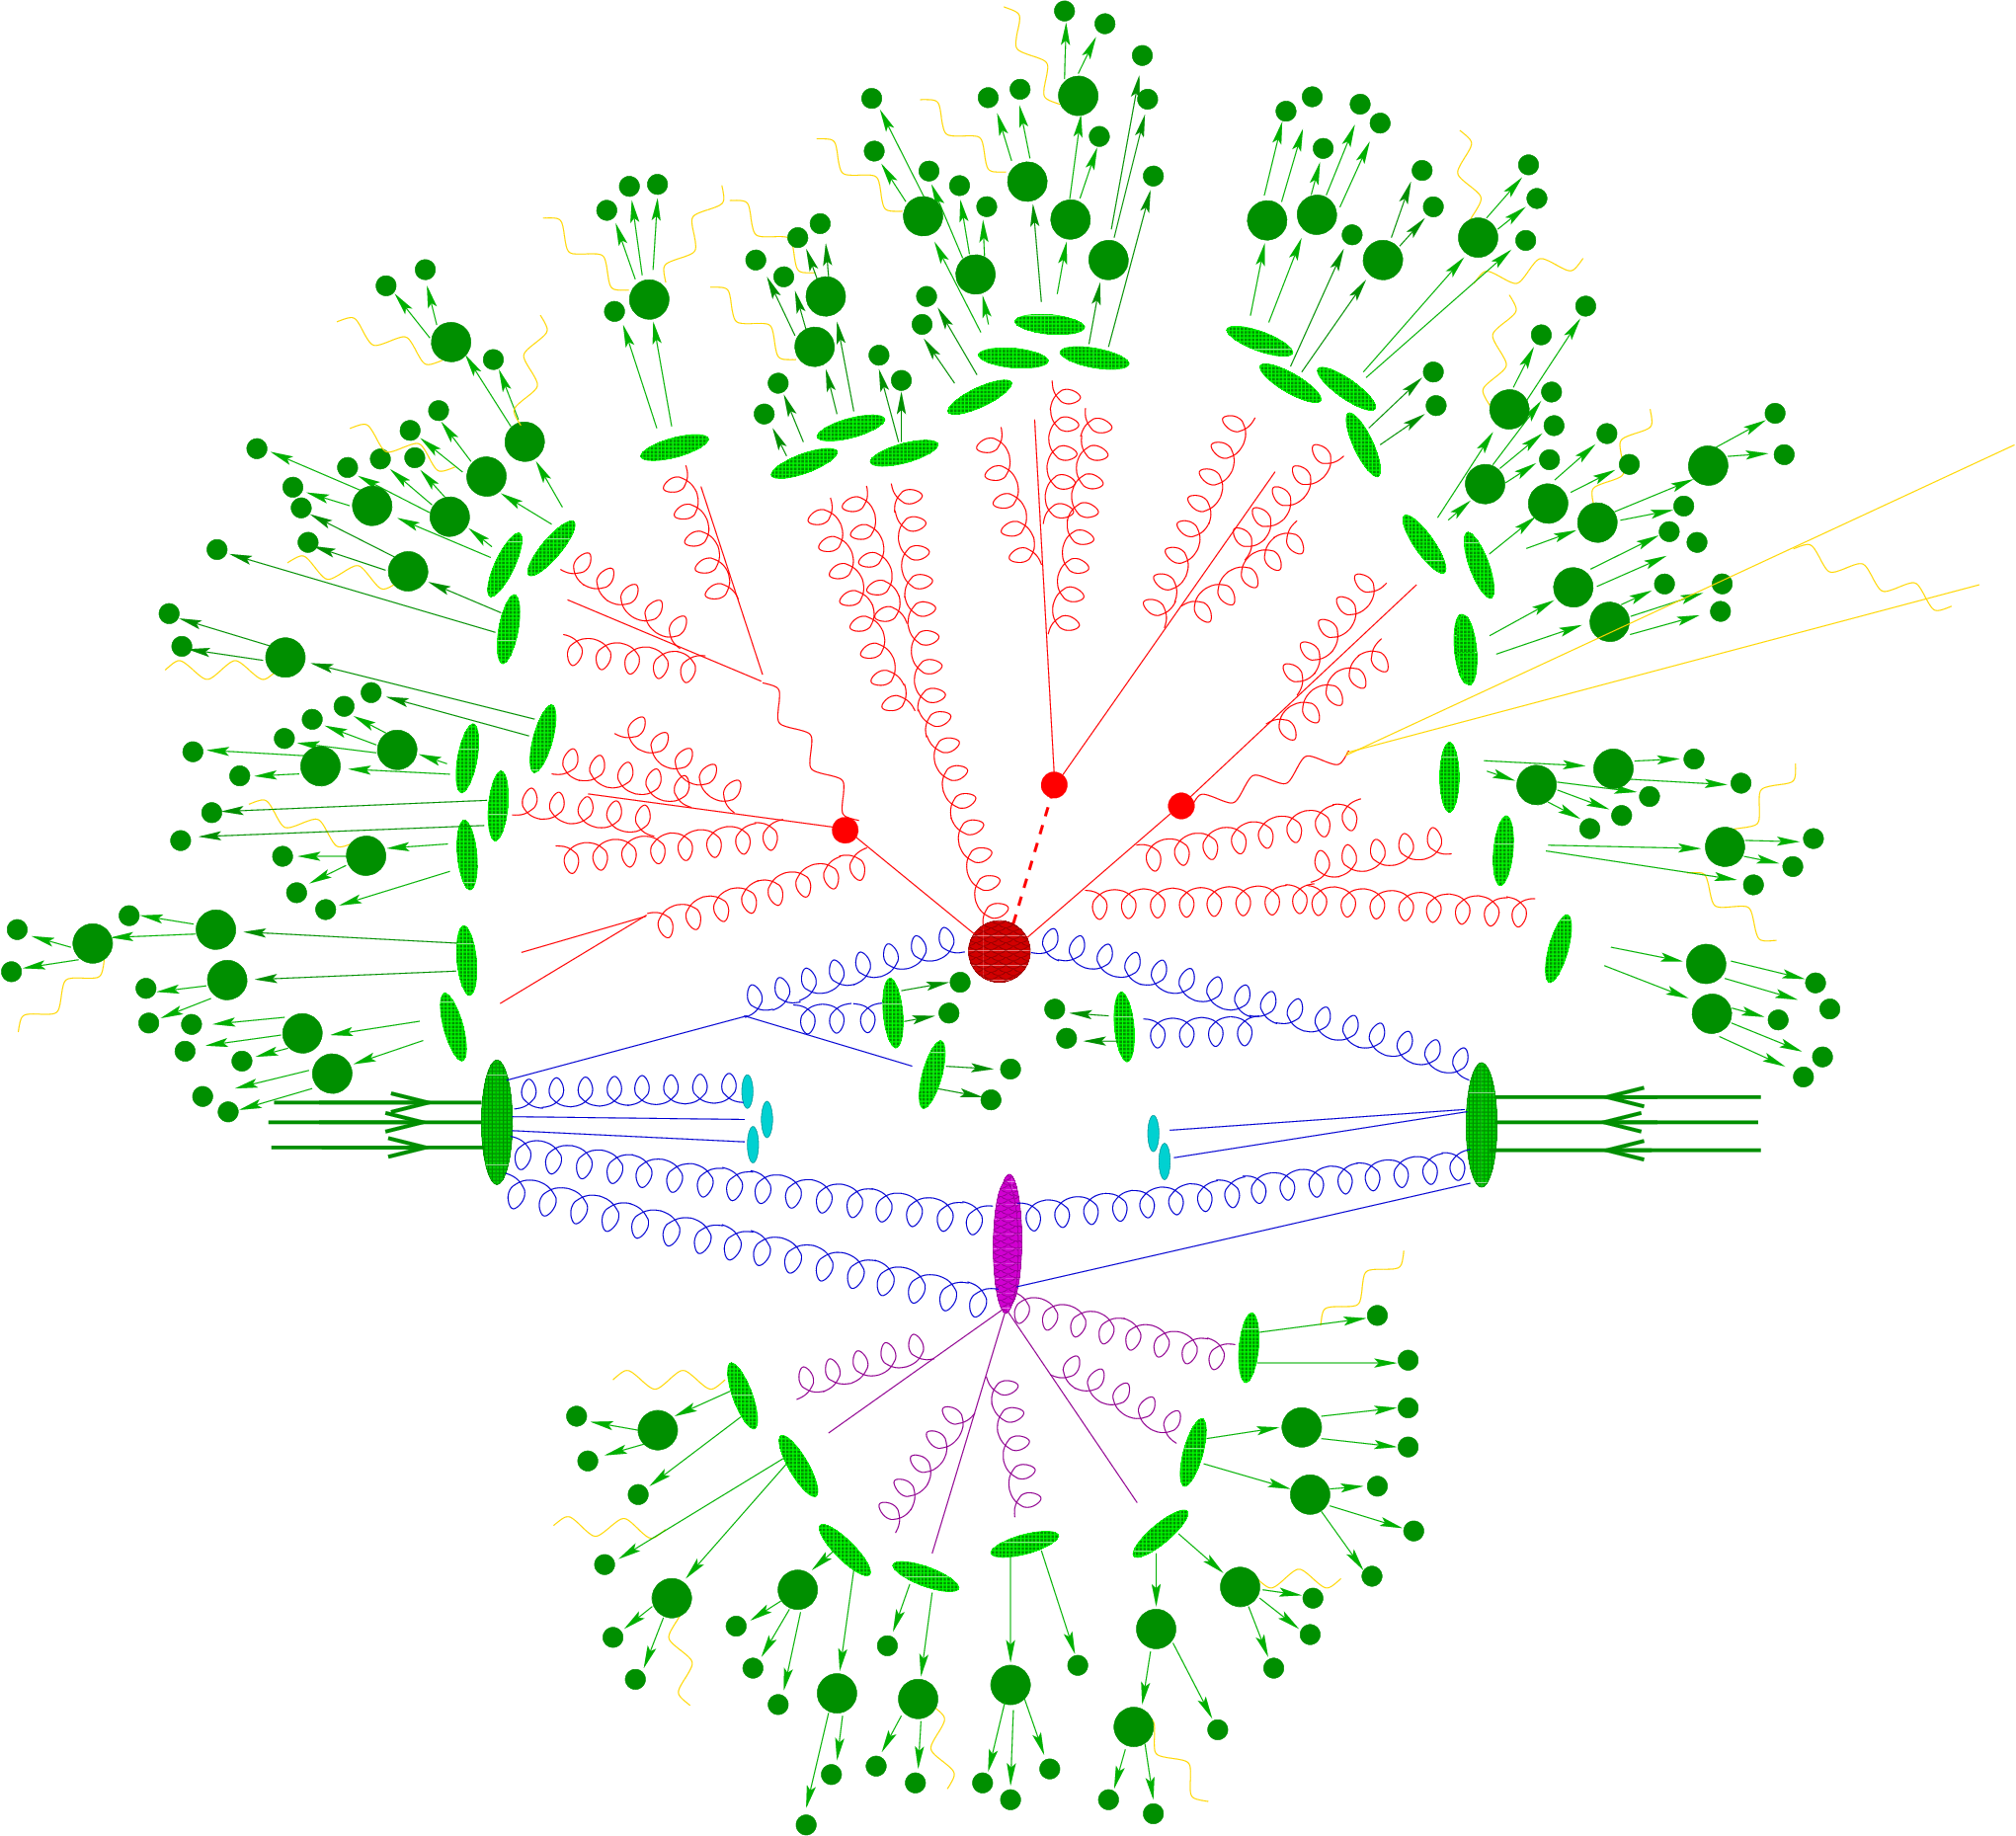
\includegraphics[width=0.65\textwidth]{figures/parton_shower.png}
	\caption{Diagram of a parton shower from a pp collison~\cite{PartonShower}.}
	\label{fig:ps}
\end{figure}

For simulations of QCD in pp collisions on the energy scales of the LHC, several methods of calculation are combined. Matrix element (ME) simulations are used for the interactions with isolated particles. The parton shower (PS) that occurs for the energy scales $\mu^2 > 1$ GeV can be used in addition to ME calculations or on its own. A depiction of a parton shower from a pp collision event is shown in Figure~\ref{fig:ps}. Additionally, there is a non-perturbative hadronization calculation at energy scales of $mu^2 < 1$ GeV. ME calculations are done with MadGraph, and PS calculations are done with Pythia and HERWIG~\cite{MadGraph,pythia8}.

Parton distribution functions (PDFs) describe the probability of a parton to be found at energy scale $Q^2$. The PDFs on the scale of the LHC are shown in Figure~\ref{fig:pdf} for the momentum fraction $x$ of the proton momentum.

\begin{figure}[h]
	\centering
	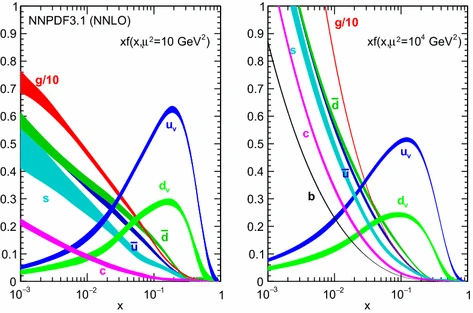
\includegraphics[width=0.65\textwidth]{figures/pdf_lhc.png}
	\caption{Diagram of a parton shower from a pp collison~\cite{pdfs}.}
	\label{fig:pdf}
\end{figure}



